\documentclass[10pt,conference]{IEEEtran}
% SANER 2027 Agentic AI4SE track: IEEEtran conference, no compsoc; 10 pages + 2 pages of references.
\usepackage{cite}
\usepackage{amsmath}
\usepackage{array}
\usepackage{url}
\usepackage{tikz}
\usetikzlibrary{arrows.meta,calc,positioning}
\usepackage[hidelinks]{hyperref}
\hypersetup{pdfauthor={},pdftitle={One Session or Five? Cohort versus Per-Item Coding-Agent Execution and Cross-Item Architectural Consistency},pdfsubject={},pdfkeywords={},pdfcreator={},pdfproducer={}}

% Every result number in the prose comes from these generated files.
% Generated by scripts/build_tables.py from data/metrics.json. Do not edit.
% Numbers only (no units or % signs). Lower bounds carry \ensuremath{\geq}.
% Reductions are percentages; ratios are independent/grouped.
\newcommand{\AcostGrouped}{9.48} % A021 platform cost USD, grouped
\newcommand{\AcostIndep}{21.51} % A021 platform cost USD, independent
\newcommand{\AcostRatio}{2.27} % A021 platform cost, independent/grouped
\newcommand{\AcostReduction}{56.0} % A021 platform cost, grouped reduction in percent
\newcommand{\AoutputGrouped}{112,377} % A021 platform output tokens, grouped
\newcommand{\AoutputIndep}{244,630} % A021 platform output tokens, independent
\newcommand{\AoutputRatio}{2.18} % A021 platform output tokens, independent/grouped
\newcommand{\AoutputReduction}{54.1} % A021 platform output tokens, grouped reduction in percent
\newcommand{\AcacheReadGrouped}{24.51} % A021 platform cache-read tokens, millions, grouped
\newcommand{\AcacheReadIndep}{45.07} % A021 platform cache-read tokens, millions, independent
\newcommand{\AcacheReadRatio}{1.84} % A021 platform cache-read tokens, independent/grouped
\newcommand{\AcacheReadReduction}{45.6} % A021 platform cache-read tokens, grouped reduction in percent
\newcommand{\AactiveMinGrouped}{61.2} % A021 active session time, minutes, grouped
\newcommand{\AactiveMinIndep}{111.4} % A021 active session time, minutes, independent
\newcommand{\AactiveRatio}{1.82} % A021 active session time, independent/grouped
\newcommand{\AactiveReduction}{45.1} % A021 active session time, grouped reduction in percent
\newcommand{\AspanMinGrouped}{61.2} % A021 wall-clock span, minutes, grouped
\newcommand{\AspanMinIndep}{292.1} % A021 wall-clock span, minutes, independent
\newcommand{\AspanHmIndep}{4:52} % A021 wall-clock span, independent, h:mm
\newcommand{\AspanRatio}{4.77} % A021 wall-clock span, independent/grouped
\newcommand{\AspanReduction}{79.1} % A021 wall-clock span, grouped reduction in percent
\newcommand{\AblockedMinIndep}{127.1} % A021 permission-block time, minutes
\newcommand{\AsessionsGrouped}{1} % A021 implementation sessions, grouped
\newcommand{\AsessionsIndep}{5} % A021 implementation sessions, independent
\newcommand{\AfailedAttemptsIndep}{2} % A021 failed attempt sessions
\newcommand{\AmodelRequestsGrouped}{\ensuremath{\geq}114} % A021 model requests (script; independent is a lower bound), grouped
\newcommand{\AmodelRequestsIndep}{\ensuremath{\geq}237} % A021 model requests (script; independent is a lower bound), independent
\newcommand{\AfileReadsGrouped}{\ensuremath{\geq}52} % A021 file reads (script; independent lower bound), grouped
\newcommand{\AfileReadsIndep}{\ensuremath{\geq}134} % A021 file reads (script; independent lower bound), independent
\newcommand{\AsearchesGrouped}{\ensuremath{\geq}53} % A021 searches (script; independent lower bound), grouped
\newcommand{\AsearchesIndep}{\ensuremath{\geq}159} % A021 searches (script; independent lower bound), independent
\newcommand{\AbuildsGrouped}{\ensuremath{\geq}16} % A021 build commands (script), grouped
\newcommand{\AbuildsIndep}{\ensuremath{\geq}34} % A021 build commands (script), independent
\newcommand{\AtestRunsGrouped}{\ensuremath{\geq}13} % A021 test-run commands (script), grouped
\newcommand{\AtestRunsIndep}{\ensuremath{\geq}15} % A021 test-run commands (script), independent
\newcommand{\AagentsReadsGrouped}{\ensuremath{\geq}1} % A021 AGENTS.md reads, grouped
\newcommand{\AagentsReadsIndep}{\ensuremath{\geq}5} % A021 AGENTS.md reads, independent
\newcommand{\AgovReadsGrouped}{\ensuremath{\geq}6} % A021 governance/planning reads, grouped
\newcommand{\AgovReadsIndep}{\ensuremath{\geq}15} % A021 governance/planning reads, independent
\newcommand{\AfirstCodeMinGrouped}{9.6} % A021 summed time to first code change, minutes, grouped
\newcommand{\AfirstCodeMinIndep}{\ensuremath{\geq}21.5} % A021 summed time to first code change, minutes, independent
\newcommand{\AcontextKGrouped}{318.8} % A021 largest end-of-session context, k tokens, grouped
\newcommand{\AcontextKIndep}{262.8} % A021 largest end-of-session context, k tokens, independent
\newcommand{\AtestsGrouped}{811} % A021 final F\# tests passed, grouped
\newcommand{\AtestsIndep}{829} % A021 final F\# tests passed, independent
\newcommand{\AtestsAddedGrouped}{19} % A021 work-group tests added (evaluation 1), grouped
\newcommand{\AtestsAddedIndep}{37} % A021 work-group tests added (evaluation 1), independent
\newcommand{\AkitDefectsGrouped}{0} % A021 kit-evaluation defect findings, grouped
\newcommand{\AkitDefectsIndep}{2} % A021 kit-evaluation defect findings, independent
\newcommand{\AmergeConflictsGrouped}{0} % A021 merges with conflicts, grouped
\newcommand{\AmergeConflictsIndep}{1} % A021 merges with conflicts, independent
\newcommand{\RtwoCostGrouped}{10.75} % R2 platform cost USD, workers, grouped
\newcommand{\RtwoCostIndep}{22.56} % R2 platform cost USD, workers, independent
\newcommand{\RtwoCostRatio}{2.10} % R2 platform cost, workers, independent/grouped
\newcommand{\RtwoCostReduction}{52.3} % R2 platform cost, workers, grouped reduction in percent
\newcommand{\RtwoOutputGrouped}{132,902} % R2 platform output tokens, workers, grouped
\newcommand{\RtwoOutputIndep}{236,654} % R2 platform output tokens, workers, independent
\newcommand{\RtwoOutputRatio}{1.78} % R2 platform output tokens, workers, independent/grouped
\newcommand{\RtwoOutputReduction}{43.8} % R2 platform output tokens, workers, grouped reduction in percent
\newcommand{\RtwoCacheReadGrouped}{27.91} % R2 platform cache-read tokens, millions, workers, grouped
\newcommand{\RtwoCacheReadIndep}{54.49} % R2 platform cache-read tokens, millions, workers, independent
\newcommand{\RtwoCacheReadRatio}{1.95} % R2 platform cache-read tokens, workers, independent/grouped
\newcommand{\RtwoCacheReadReduction}{48.8} % R2 platform cache-read tokens, workers, grouped reduction in percent
\newcommand{\RtwoActiveMinGrouped}{55.9} % R2 active session time, workers, minutes, grouped
\newcommand{\RtwoActiveMinIndep}{100.5} % R2 active session time, workers, minutes, independent
\newcommand{\RtwoActiveRatio}{1.80} % R2 active session time, workers, independent/grouped
\newcommand{\RtwoActiveReduction}{44.4} % R2 active session time, workers, grouped reduction in percent
\newcommand{\RtwoSpanMinGrouped}{55.9} % R2 wall-clock span, workers, minutes, grouped
\newcommand{\RtwoSpanMinIndep}{133.3} % R2 wall-clock span, workers, minutes, independent
\newcommand{\RtwoSpanRatio}{2.38} % R2 wall-clock span, workers, independent/grouped
\newcommand{\RtwoSpanReduction}{58.1} % R2 wall-clock span, workers, grouped reduction in percent
\newcommand{\RtwoCostInclOrchIndep}{26.05} % R2 platform cost USD, independent incl. orchestrator
\newcommand{\RtwoOrchCostIndep}{3.49} % R2 independent-arm orchestrator cost USD
\newcommand{\RtwoCostInclOrchRatio}{2.4224} % R2 platform cost incl. orchestrator, independent/grouped
\newcommand{\RtwoCostInclOrchReduction}{58.72} % R2 platform cost incl. orchestrator, grouped reduction in percent
\newcommand{\RtwoOutputInclOrchRatio}{1.9781} % R2 output tokens incl. orchestrator, independent/grouped
\newcommand{\RtwoOutputInclOrchReduction}{49.45} % R2 output tokens incl. orchestrator, grouped reduction in percent
\newcommand{\RtwoCacheReadInclOrchRatio}{2.2557} % R2 cache-read incl. orchestrator, independent/grouped
\newcommand{\RtwoCacheReadInclOrchReduction}{55.67} % R2 cache-read incl. orchestrator, grouped reduction in percent
\newcommand{\RtwoElapsedGrouped}{0h55m53s} % R2 elapsed as reported, grouped
\newcommand{\RtwoElapsedIndep}{2h23m35s} % R2 elapsed as reported, independent
\newcommand{\RtwoElapsedRatio}{2.5693} % R2 elapsed as reported (wall-clock incl. orchestration), independent/grouped
\newcommand{\RtwoElapsedReduction}{61.08} % R2 elapsed as reported (wall-clock incl. orchestration), grouped reduction in percent
\newcommand{\RtwoSessionsGrouped}{1} % R2 implementation sessions, grouped
\newcommand{\RtwoSessionsIndep}{5} % R2 implementation sessions, independent
\newcommand{\RtwoModelRequestsGrouped}{\ensuremath{\geq}126} % R2 model requests (script), grouped
\newcommand{\RtwoModelRequestsIndep}{\ensuremath{\geq}343} % R2 model requests (script), independent
\newcommand{\RtwoFileReadsGrouped}{\ensuremath{\geq}69} % R2 file reads (script), grouped
\newcommand{\RtwoFileReadsIndep}{\ensuremath{\geq}185} % R2 file reads (script), independent
\newcommand{\RtwoSearchesGrouped}{\ensuremath{\geq}98} % R2 searches (script), grouped
\newcommand{\RtwoSearchesIndep}{\ensuremath{\geq}208} % R2 searches (script), independent
\newcommand{\RtwoAgentsReadsGrouped}{\ensuremath{\geq}2} % R2 AGENTS.md reads, grouped
\newcommand{\RtwoAgentsReadsIndep}{\ensuremath{\geq}8} % R2 AGENTS.md reads, independent
\newcommand{\RtwoGovReadsGrouped}{\ensuremath{\geq}8} % R2 governance/planning reads, grouped
\newcommand{\RtwoGovReadsIndep}{\ensuremath{\geq}34} % R2 governance/planning reads, independent
\newcommand{\RtwoFirstCodeMinGrouped}{9.4} % R2 summed time to first code change, minutes, grouped
\newcommand{\RtwoFirstCodeMinIndep}{34.2} % R2 summed time to first code change, minutes, independent
\newcommand{\RtwoTestsGrouped}{819} % R2 final F\# tests passed, grouped
\newcommand{\RtwoTestsIndep}{839} % R2 final F\# tests passed, independent
\newcommand{\RtwoTestsAddedGrouped}{27} % R2 net F\# tests added vs baseline, grouped
\newcommand{\RtwoTestsAddedIndep}{47} % R2 net F\# tests added vs baseline, independent
\newcommand{\RtwoDefectsGrouped}{2} % R2 confirmed acceptance defects, grouped
\newcommand{\RtwoDefectsIndep}{2} % R2 confirmed acceptance defects, independent
\newcommand{\RtwoMergeConflictsGrouped}{0} % R2 merges with conflicts, grouped
\newcommand{\RtwoMergeConflictsIndep}{2} % R2 merges with conflicts, independent
\newcommand{\BaselineTests}{792} % F\# tests at the shared baseline
\newcommand{\AcostReductionExclFailed}{46.4} % A021 platform cost, grouped reduction in percent, excluding failed attempts
\newcommand{\AactiveReductionExclFailed}{30.7} % A021 active session time, grouped reduction in percent, excluding failed attempts

% Generated by scripts/build_architecture_table.py from data/architecture-findings.json and data/metrics.json. Do not edit.
\newcommand{\ArchDimensions}{eight} % rubric dimensions
\newcommand{\ArchFindings}{32} % coded findings (study x arm x dimension)
\newcommand{\ArchCitations}{100} % code citations verified
\newcommand{\ArchFalsificationAttempts}{12} % falsification attempts


\newcommand{\G}{G}
\newcommand{\I}{I}

\begin{document}

\title{One Session or Five? Cohort versus Per-Item Coding-Agent Execution and Cross-Item Architectural Consistency: A Case Study with a Close Replication}

\author{\IEEEauthorblockN{Anonymous Author(s)}\IEEEauthorblockA{Anonymous Institution(s)}}

\maketitle

\begin{abstract}
Coding agents are usually given one work item per fresh session, even when several items share design decisions. We compare two ways of executing the same five coupled work items in an F\#/.NET command-line tool: \emph{cohort execution}, one session that implements all five items after writing and committing a mandated cross-item analysis, and \emph{per-item execution}, five fresh sessions run serially on one shared branch with prompts that never mention the cohort. % CLAIM: C01
The cohort arm differs in both retained context and the mandated analysis, so we compare these two treatments as bundles and do not attribute effects to shared context alone. % CLAIM: C02
An original study and an internal close replication each ran one execution per arm from a common baseline. % CLAIM: C08
On like-for-like worker-only figures, per-item execution used \AcostRatio$\times$ the platform cost of cohort execution in the original study and \RtwoCostRatio$\times$ in the replication (reductions of \AcostReduction\% and \RtwoCostReduction\%), and summed active session time was \AactiveReduction\% and \RtwoActiveReduction\% lower for the cohort arm. % CLAIM: C11 C13 C12 C14
On an \ArchDimensions-dimension architecture rubric applied after unblinding by one auditor, the cohort arm was more unified on \ArchAGroupedMore{} dimensions (\ArchAGroupedBeh{} behavioral) in the original study and on \ArchRtwoGroupedMore{} (\ArchRtwoGroupedBeh{} behavioral) in the replication. % CLAIM: C21 C22
Per-item execution was better on checkpoint ownership validation in both studies, reused more of the existing baseline rules, and added more tests. Local correctness was mixed, with confirmed defects in both arms. % CLAIM: C23 C24 C30 C34
The original evaluations were not effectively blind; only the replication's cross-vendor evaluation was blind, by the evaluator's own report. % CLAIM: C06 C07
We report a trade-off between resources and cross-item consistency on one side and local correctness on the other, not a general advantage, and provide an anonymous artifact with prompts, patches, metrics and analysis scripts.
\end{abstract}

\begin{IEEEkeywords}
coding agents, agentic software engineering, execution granularity, architectural consistency, replication, case study
\end{IEEEkeywords}

% ======================================================================
\section{Introduction}\label{sec:intro}

Agentic coding tools are increasingly used to implement backlog items with little supervision~\cite{li2025aiteammates,watanabe2025agentic}. A common way to use them is one work item per fresh session. That is also the unit of evaluation in issue-resolution benchmarks, where every instance is solved in isolation~\cite{jimenez2024swebench,yang2024sweagent}. Many backlogs, however, contain clusters of items that share a domain model, a persistence format, validation rules and command conventions. When each item is solved in a separate session, every session has to rebuild the shared context and may settle the shared invariants in its own way. One longer session over the whole cluster may make those decisions once, but it may also lose per-item detail as its context grows~\cite{liu2024lost,laban2025lost}.

Prior work already shows that how coupled work is divided among agents changes outcomes. Splitting two potentially conflicting features across two communicating agents lowered success compared with one agent doing both~\cite{khatua2026cooperbench}, and collaboration topology moved quality, cost and time~\cite{ren2026coordination}. We do not claim that execution granularity mattering is new. Our object is narrower and common in practice: \emph{serial, non-communicating fresh sessions on one branch} versus \emph{one cohort session}, on real repository work, with \emph{cross-item architectural unification} measured alongside resource use and per-item correctness.

We studied five coupled work items in an F\#/.NET command-line tool. They added the five verbs of one new command family (create, show, add, remove and checkpoint a group of work items). Two arms started from the same baseline commit. In \emph{cohort execution} (the grouped arm, \G), one session read all five items and the tool's planner explanation of the cohort, wrote and committed a cross-item analysis before changing any code, and then implemented the items one after another in the same session. In \emph{per-item execution} (the independent arm, \I), five fresh sessions ran serially on one shared branch. Each received a prompt for its own item that did not say the items were related. % CLAIM: C01
The grouped arm therefore differs from the independent arm in at least two ways: it retains context, and it was instructed to analyze the cohort before coding. Our data cannot separate these components, so every effect we report is an effect of the bundle. % CLAIM: C02
We ran the comparison twice: the original study (A021), under a protocol frozen before the arms started, and an internal close replication (R2) with new executions and a different evaluator. % CLAIM: C04 C08

The contributions are:
(i) a controlled comparison of cohort versus per-item execution of one coupled five-item cohort from a common baseline, with the treatment confound stated;
(ii) a symmetric \ArchDimensions-dimension measurement of cross-item architectural unification with code citations and runtime probes, which gives the dimensions where per-item execution was better the same prominence;
(iii) worker-only resource measures and lower-bound repeated-context counts;
(iv) an execution replication with a replication matrix that marks each outcome as reproduced, mixed, not reproduced or not tested; and
(v) a full disclosure of deviations, threats and corrections, with an anonymous artifact.
The results are descriptive (one execution per arm per study). They do not establish a causal mechanism or a general advantage for either mode.

% ======================================================================
\section{Background and Related Work}\label{sec:related}

\textbf{Agents and task units.} Repository-level benchmarks evaluate one issue or feature per instance~\cite{jimenez2024swebench,li2025feabench,deng2025swebenchpro}, and agent scaffolds are compared on those instances~\cite{yang2024sweagent,wang2025openhands,zhang2024autocoderover,xia2025agentless}. SWE-Bench-CL orders issues in time and studies transfer through an external memory~\cite{joshi2025swebenchcl}. EvoCode-Bench runs multi-round tasks in a persistent workspace and finds that carried-over state can propagate earlier errors~\cite{shen2026evocode}, which is evidence against assuming that retained state helps.

\textbf{Partitioning coupled work.} CooperBench is the closest prior work: one agent implementing two features outperformed two communicating agents implementing one each~\cite{khatua2026cooperbench}. MSEval varies collaboration topology~\cite{ren2026coordination}. CAID finds that isolated workspaces with a manager and test-verified merging can beat a single agent~\cite{geng2026caid}, and shared files can carry coordination between agents~\cite{destefanis2026coordinate}. Multi-agent failure taxonomies include inter-agent misalignment~\cite{cemri2025why}, and role-based pipelines reduce inconsistencies from naive chaining~\cite{hong2024metagpt,qian2024chatdev}. Agents that solve tasks independently repeat mistakes that experience reuse can avoid~\cite{qian2024experiential}. Practitioner reports argue that sub-agents that cannot see each other's decisions produce inconsistent work~\cite{yan2025dontbuild,hadfield2025multiagent}. Unlike these studies, our split sessions run one after another, do not communicate, and see earlier work only through the shared branch, and we measure whether shared invariants were resolved once or repeatedly.

\textbf{Grouping inside one context.} Batch prompting and multi-task inference reduce cost by placing several tasks in one call, sometimes without loss of quality~\cite{cheng2023batch,son2024multitask}. Plan-then-execute prompting~\cite{wang2023plan} is related to our grouped arm's mandated analysis, which is one reason the treatment is a bundle. Retrieval is the usual way a fresh session rebuilds shared state~\cite{zhang2023repocoder}. Coherence debt describes how missing coupled facts lead agents to guess~\cite{mohammadi2026coherence}. Context management within a session is itself a strong cost lever~\cite{lindenbauer2025complexity,rajasekaran2025context,packer2023memgpt}, and reviewing in a fresh session can find errors that same-session review misses~\cite{song2026crosscontext}.

\textbf{Cost.} Agent evaluations should report cost together with accuracy~\cite{kapoor2025agents}. Token use in agentic coding is dominated by input and varies greatly between runs of the same task~\cite{bai2026tokens,salim2026tokenomics}. This variation bounds any interpretation of a single execution per arm.

\textbf{Architecture and method.} Our consistency outcome draws on work on architectural erosion and drift~\cite{perry1992foundations,desilva2012controlling,li2022understanding}, on decomposition along design decisions~\cite{parnas1972criteria} and on coordination costs when work is split~\cite{herbsleb1999splitting}. We follow case-study guidance~\cite{runeson2009guidelines,ralph2020empirical}, use experiment terminology~\cite{wohlin2012experimentation} and the replication taxonomy of G\'omez et al.~\cite{gomez2014understanding,shull2008role,baldassarre2014replication}, and report model, runtime and evaluator roles as recommended for LLM-based SE studies~\cite{wagner2025towards,baltes2025guidelines,sallou2024breaking}. Evaluators that are themselves models have documented biases~\cite{zheng2023judging,wang2024fair,he2025judgese}.

\textbf{Novelty.} In the sources we examined, no study measured whether separate agent sessions converged on the same cross-cutting decisions (one store, one admission rule, one error contract), together with cost and per-item correctness, on one real cohort. % CLAIM: C45
Our search covered recent preprints only incompletely, and several entries were verified only at abstract level.

% ======================================================================
\section{Research Questions}\label{sec:rq}

\begin{itemize}
\item \textbf{RQ1 (resources).} How do platform cost, active session time, tokens and repeated context acquisition differ between cohort and per-item execution?
\item \textbf{RQ2 (architectural consistency).} Which arm resolves shared cross-item concerns in a more unified way, and on which dimensions is the per-item arm better?
\item \textbf{RQ3 (local correctness).} What trade-off appears between cross-item consistency and per-item acceptance fidelity, tests and defects?
\item \textbf{RQ4 (replication).} Does a second execution from the same baseline repeat the direction of the RQ1--RQ3 results?
\item \textbf{RQ5 (boundary).} Which results remain after the treatment confound, the evaluation and orchestration deviations, and stale checkouts are taken into account?
\end{itemize}
The four outcome families (resources, architectural consistency, local correctness and reproducibility) are reported separately. We do not combine them into a quality score, because no weighting was defined before the evaluation.

% ======================================================================
\section{Subject System and Cohort}\label{sec:subject}

The subject system is an F\#/.NET command-line tool that governs repository work items: it records items, their lifecycle (start, checkpoint, complete) and attribution, and includes a read-only planner that groups related items. The cohort consists of five items that together add a \texttt{work group} command family: \emph{create} (item 1), \emph{show} (2), \emph{add} (3), \emph{remove} (4) and \emph{checkpoint} (5). The acceptance criteria were in the item descriptions before either arm started. The items share a persistence model, a member-admission rule (which items may join a group, including an execution-repository rule), a member classification, checkpoint ownership rules, an error and JSON contract, and a mutation path. At the baseline the planner rated the cohort as high affinity, rated every pair of items as conflicting, and recommended a safe concurrency of one, so the per-item sessions had to run serially. % CLAIM: C05
The cohort was authored by the same agent lineage that designed the experiment, and it extends the planner's own grouping feature (Section~\ref{sec:threats}). % CLAIM: C41

% ======================================================================
\section{Experimental Design}\label{sec:design}

\begin{figure}[t]
\centering
% Study design flow (Fig. 1). TikZ; no data values. Explicit coordinates (column width).
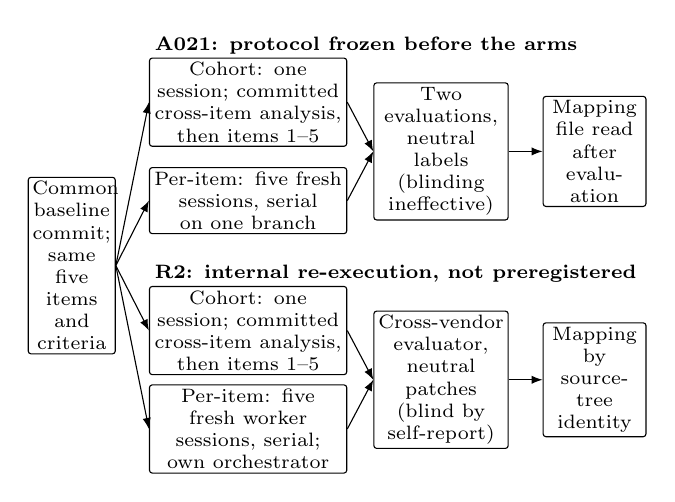
\begin{tikzpicture}[
  font=\scriptsize,
  box/.style={draw, rounded corners=1pt, align=center, inner sep=1.5pt, minimum height=6mm},
  arm/.style={box, anchor=west, text width=24mm},
  eval/.style={box, anchor=west, text width=16mm},
  rev/.style={box, anchor=west, text width=12mm},
  study/.style={font=\scriptsize\bfseries, anchor=west},
  arr/.style={-{Latex[length=1.4mm]}, thin}]
  % rows: A021 cohort, A021 per-item, R2 cohort, R2 per-item
  \node[study] at (1.55, 0.72) {A021: protocol frozen before the arms};
  \node[arm] (ag) at (1.6, 0.0) {Cohort: one session; committed cross-item analysis, then items 1--5};
  \node[arm] (ai) at (1.6, -1.25) {Per-item: five fresh sessions, serial on one branch};
  \node[eval] (ae) at (4.45, -0.625) {Two evaluations, neutral labels (blinding ineffective)};
  \node[rev] (ar) at (6.6, -0.625) {Mapping file read after evaluation};
  \node[study] at (1.55, -2.18) {R2: internal re-execution, not preregistered};
  \node[arm] (rg) at (1.6, -2.9) {Cohort: one session; committed cross-item analysis, then items 1--5};
  \node[arm] (ri) at (1.6, -4.15) {Per-item: five fresh worker sessions, serial; own orchestrator};
  \node[eval] (re) at (4.45, -3.525) {Cross-vendor evaluator, neutral patches (blind by self-report)};
  \node[rev] (rr) at (6.6, -3.525) {Mapping by source-tree identity};
  % common baseline
  \node[box, text width=10mm] (b) at (0.62, -2.075) {Common baseline commit; same five items and criteria};
  \foreach \t in {ag, ai, rg, ri} \draw[arr] (b.east) -- (\t.west);
  \foreach \s/\e in {ag/ae, ai/ae, rg/re, ri/re} \draw[arr] (\s.east) -- (\e.west);
  \draw[arr] (ae) -- (ar);
  \draw[arr] (re) -- (rr);
\end{tikzpicture}

\caption{Design of both studies. All four arms branch from the same baseline commit. Each study has one execution per arm. In A021 the arm labels were visible to the evaluators (Section~\ref{sec:design-eval}).}
\label{fig:design}
\end{figure}

Fig.~\ref{fig:design} summarizes both studies. All four arms branch from the same baseline commit, implement the same five items against the same criteria and repository instructions, and were not merged before evaluation. % CLAIM: C03
All implementation sessions used one fixed Claude model through the Claude Code remote runtime; the model identifier is recorded per session in the artifact. Each session ran in its own container and workspace. % CLAIM: C10
Every prompt carried the same instrumentation note (toolchain setup, timestamps, a metrics script, no pull requests).

\subsection{Treatments}\label{sec:design-treatments}
\textbf{Cohort execution (\G).} One session receives all five items. Its prompt requires it to read every item and the planner's explanation of the group, then, \emph{before changing any code}, to write and commit an analysis covering common architecture, shared invariants, conflicting requirements, order, reusable abstractions, common tests and the risks of solving each item separately. It then implements each item under its own lifecycle, labels shared changes as group infrastructure, and checkpoints after milestones. \textbf{Per-item execution (\I).} Five fresh sessions run one after another in the planner's order on one branch. Each sees the repository, including earlier items' pushed commits, but none of the earlier sessions' reasoning. Each prompt names only its own item. It does not mention the cohort, show the planner output, or ask for consistency with other items. % CLAIM: C01
The prompts thus differ in more than session count: only \G{} is given the group framing, the planner explanation, the committed design step, the shared-infrastructure labelling and milestone checkpoints. We therefore compare \emph{cohort execution with a mandated up-front cross-item analysis} against \emph{uninstructed per-item execution}. A design that separates retained context from the analysis step (for example a third arm with a shared analysis and per-item sessions) is future work. % CLAIM: C02

\subsection{A021: original study}
The protocol, prompts and planner predictions were committed before the arms branched, and server-side push times confirm that they were not edited afterwards. % CLAIM: C04
The per-item arm needed seven sessions: item 4 failed twice before a third attempt completed it (Table~\ref{tab:deviations}). % CLAIM: C37

\subsection{R2: internal close replication}
R2 reused the baseline, cohort, criteria, organization and implementing model, and produced new executions of both arms. It changed the evaluator. Following G\'omez et al.~\cite{gomez2014understanding}, it is an \emph{internal close (operational) replication}. It was not separately preregistered. Its prompts were fuller owner-written versions of the A021 prompts and were not archived. Its designer knew interim A021 results, and the R2 grouped analysis included headings for the dimensions on which the evaluator later scored the arms. % CLAIM: C08 C09
The R2 per-item arm also had its own orchestrator session, which created the five workers and waited for each one. The cohort arm had none. % CLAIM: C38

\subsection{Evaluation and unblinding}\label{sec:design-eval}
\textbf{A021.} Two evaluations were made under neutral arm labels, but neither was effectively blind. The first evaluator received full branches whose commit subjects named the arm and reported reading them. The second evaluator reported that it knew the mapping before it read any code. The first evaluator ran on the same model as the implementers (the second evaluator's model was not recorded), and its brief asked explicitly whether each arm had one model of the declared group. We therefore use the A021 evaluations only for structural facts that the architecture audit re-verified in code. % CLAIM: C06 C40
\textbf{R2.} A different vendor's model (OpenAI ChatGPT) evaluated squashed, neutrally named patches whose checksums had been recorded beforehand. The evaluation was pushed before the unblinding. Blindness rests on the evaluator's self-report: it could technically reach the arm branches, and the mapping was later recovered from source-tree identity because the salt of the pre-evaluation mapping commitment was lost. The same evaluator later unblinded, computed the ratios and updated the hypothesis record. % CLAIM: C07 C39

% ======================================================================
\section{Measures}\label{sec:measures}

\textbf{Resources.} \emph{Platform cost} and token counts (output, cache-read, cache-write, uncached input) are the runtime's whole-session usage records. \emph{Workers} are all sessions that worked on an arm's items, including failed attempts. They exclude orchestration and evaluator sessions. The worker-only figures are our primary, like-for-like definition across both studies. % CLAIM: C11 C13
We use four time definitions and never mix them. A \emph{session span} runs from a session's creation to its end; a session blocked on a permission prompt ends at the block. \emph{Summed active session time} is the sum of the spans of an arm's workers, and it is our primary time measure. A \emph{wall-clock span} runs from the first start to the last end of the included sessions and includes the gaps between sessions. The R2 record's ``elapsed'' is a wall-clock span from the common arm start to the per-item orchestrator's last update. \emph{Blocked time} is the time a session waited on a permission prompt. % CLAIM: C12 C16
Wall-clock spans are reported only as secondary figures, and we never compare a span with a summed time.

\textbf{Repeated context.} Each session ran a transcript script that counted model requests, file reads, searches, builds, test runs, reads of the repository instructions and governance documents, and time to first code change. Each session ran the script before its final steps, and the two failed A021 attempts have no script output, so all of these counts are \emph{lower bounds}. Ratios of lower bounds are not bounds themselves. % CLAIM: C18
Compactions were counted from the transcripts.

\textbf{Architectural consistency.} Eight dimensions, D1--D8 (Table~\ref{tab:architecture}): persistence model, member admission (create vs.\ add), member classification (show vs.\ checkpoint), checkpoint ownership validation, error/JSON/exit contract, mutation and concurrency model, reuse of baseline rules, and incompatible duplicates inside the feature.

\textbf{Local correctness.} The tests added and passing, as counted by the evaluators; the per-criterion verdicts and confirmed acceptance defects of each evaluation; and design risks. We keep these separate. A larger number of tests is not evidence of better tests.

% ======================================================================
\section{Analysis Method}\label{sec:analysis}

\textbf{Descriptive comparison.} For each measure we report both raw values, the ratio I/G and the reduction $(I-G)/I$, and whether the value is complete or a lower bound. With one execution per arm in each study, and items within an execution that are not independent samples, we compute no inferential statistics and do not average across studies.

\textbf{Architecture rubric and coding rule.} Each arm receives one category per dimension: \emph{unified} (one rule serves every verb, with the same behavior on the same input), \emph{duplicated-compatible} (several representations, but no reachable input produces contradictory behavior), \emph{divergent} (concrete code or runtime evidence shows different behavior for the same input), \emph{missing}, or \emph{not assessable}. Following the analysis plan, a dimension is \emph{divergent} only when concrete evidence shows different behavior; a difference in organization alone never qualifies. Every finding cites commit, path, line range and symbol and is marked as observed, evaluated or inferred. A script checks that each cited symbol occurs in its cited range. The audit coded \ArchFindings{} findings with \ArchCitations{} code citations. It built all four heads and ran runtime probes against each arm's own binary, including a concurrent-create probe. It also tested \ArchFalsificationAttempts{} statements made in the original records against the code. % CLAIM: C29
The rubric was applied after unblinding by one auditor, an AI agent from the same organization. Inter-rater reliability was not measured. % CLAIM: C29

\textbf{Sensitivity analyses} (defined in the analysis plan after the executions and before this manuscript was drafted).
\emph{S1}, excluding the failed A021 attempts from the per-item arm.
\emph{S2}, using summed active session time instead of wall-clock spans that include orchestration gaps.
\emph{S3}, treating the stale-start items as confounders: findings that depend on a stale item are flagged and the contrast is recomputed without them.
\emph{S4}, setting test counts aside and reading only the defect and verdict evidence.
\emph{S5}, asking whether lower cost alone could explain the architectural result. It cannot, because the architecture outcome is code-based and separately evidenced. Cost cannot establish a mechanism.

% ======================================================================
\section{Results: Original Study (A021)}\label{sec:results}

% Generated by scripts/build_tables.py from data/metrics.json. Do not edit.
\begin{table}[t]
\centering
\scriptsize
\caption{A021 resources and repeated work, grouped versus independent execution}
\label{tab:resources-a021}
\begin{tabular}{@{}p{0.44\columnwidth}rrrr@{}}
\hline
Measure & Grouped & Indep. & I/G & Red.\ (\%) \\
\hline
Implementation sessions & 1 & 5 & -- & -- \\
Failed attempt sessions & 0 & 2 & -- & -- \\
Cost, platform (USD) & 9.48 & 21.51 & 2.27 & 56.0 \\
Output tokens, platform (k) & 112.4 & 244.6 & 2.18 & 54.1 \\
Cache-read tokens, platform (M) & 24.51 & 45.07 & 1.84 & 45.6 \\
Cache-write tokens, platform (k) & 290.8 & 950.6 & 3.27 & 69.4 \\
Uncached input tokens, platform & 234 & 658 & 2.81 & 64.4 \\
Active session time, sum (min) & 61.2 & 111.4 & 1.82 & 45.1 \\
Wall-clock span, first start to last end (h:mm) & 1:01 & 4:52 & 4.77 & 79.1 \\
Blocked on a permission prompt (min) & -- & 127.1 & -- & -- \\
Largest end-of-session context (k tokens) & 318.8 & 262.8 & -- & -- \\
Model requests, script & $\geq$114 & $\geq$237 & 2.08$^{\ast}$ & 51.9$^{\ast}$ \\
File reads, script & $\geq$52 & $\geq$134 & 2.58$^{\ast}$ & 61.2$^{\ast}$ \\
Searches, script & $\geq$53 & $\geq$159 & 3.00$^{\ast}$ & 66.7$^{\ast}$ \\
Build commands, script & $\geq$16 & $\geq$34 & 2.12$^{\ast}$ & 52.9$^{\ast}$ \\
Test-run commands, script & $\geq$13 & $\geq$15 & 1.15$^{\ast}$ & 13.3$^{\ast}$ \\
AGENTS.md reads, script & $\geq$1 & $\geq$5 & 5.00$^{\ast}$ & 80.0$^{\ast}$ \\
Governance/planning document reads, script & $\geq$6 & $\geq$15 & 2.50$^{\ast}$ & 60.0$^{\ast}$ \\
Time to first code change, summed (min) & 9.6 & $\geq$21.5 & 2.24$^{\ast}$ & 55.3$^{\ast}$ \\
Compactions & 0 & $\geq$0 & -- & -- \\
Merges with conflicts & 0 & 1 & -- & -- \\
Commits after baseline & 18 & 13 & -- & -- \\
\hline
\end{tabular}

\vspace{2pt}\parbox{\columnwidth}{\scriptsize Grouped: one session. Independent: five item sessions plus two failed item-04 attempts; the shared orchestrator and the evaluator are excluded. Platform figures are whole-session get\_session usage. ``Script'' figures come from each session's own session\_metrics.py run, taken before its final steps; the independent arm has none for the two failed attempts. I/G is the independent/grouped ratio; Red.\ is (independent$-$grouped)/independent. $\geq$: lower bound. $^{\ast}$: computed from partial or lower-bound operands, so it is not a bound on the true value. Active time ends a blocked session at the block; the wall-clock span includes orchestration gaps and the block. End-of-session context approximates the peak (no compactions).}
\end{table}


\subsection{RQ1: Resources}
Worker-only platform cost was \$\AcostGrouped{} for \G{} and \$\AcostIndep{} for \I, so \I{} cost \AcostRatio$\times$ as much in this execution, a reduction of \AcostReduction\% for \G. % CLAIM: C11
Summed active session time was \AactiveMinGrouped{} versus \AactiveMinIndep{} minutes (reduction \AactiveReduction\%). % CLAIM: C12
\G{} also used fewer output tokens (\AoutputGrouped{} vs.\ \AoutputIndep; reduction \AoutputReduction\%) and fewer cache-read tokens (\AcacheReadGrouped{} vs.\ \AcacheReadIndep{} million; reduction \AcacheReadReduction\%) (Table~\ref{tab:resources-a021}). % CLAIM: C15
\emph{S1:} without the \AfailedAttemptsIndep{} failed item-4 attempts, the reductions are \AcostReductionExclFailed\% for cost and \AactiveReductionExclFailed\% for active time. The direction is unchanged, and the size depends on whether the failed attempts are counted. % CLAIM: C17
\emph{S2:} the wall-clock span of \I{} was \AspanHmIndep{} (h:mm). It includes orchestration gaps and \AblockedMinIndep{} minutes during which a session was blocked on a permission prompt, so it describes the conditions of this run rather than the execution mode. We do not use it as a primary figure. % CLAIM: C16
Repeated-context counts were lower for \G, all as lower bounds: model requests \AmodelRequestsGrouped{} vs.\ \AmodelRequestsIndep, file reads \AfileReadsGrouped{} vs.\ \AfileReadsIndep, searches \AsearchesGrouped{} vs.\ \AsearchesIndep, and reads of the repository instructions \AagentsReadsGrouped{} vs.\ \AagentsReadsIndep. % CLAIM: C18
Part of this difference follows from the design: every fresh session is told to follow the repository instructions, so it reads them once. % CLAIM: C19
No session in either arm compacted its context. % CLAIM: C20

% Generated by scripts/build_architecture_table.py from data/architecture-findings.json and data/metrics.json. Do not edit.
\begin{table}[t]
\centering
\scriptsize
\setlength{\tabcolsep}{3pt}
\caption{Architecture rubric: category per arm and direction per study}
\label{tab:architecture}
\begin{tabular}{@{}p{0.40\columnwidth}cccc@{}}
\hline
 & \multicolumn{2}{c}{A021} & \multicolumn{2}{c}{R2} \\
Dimension & G/I & Dir. & G/I & Dir. \\
\hline
D1 Persistence/store model & U/DC & G & U/DC & G \\
D2 Member admission (create vs.\ add) & U/Dv & G$^{b}$ & U/Dv & G$^{b}$ \\
D3 Member classification (show vs.\ checkpoint) & U/Dv$^{\dagger}$ & G$^{b}$ & Dv/Dv$^{\dagger}$ & eq \\
D4 Checkpoint ownership validation & Mi/U$^{\dagger}$ & I$^{b}$ & Mi/U & I$^{b}$ \\
D5 Error/JSON/exit contract & U/Dv & G$^{b}$ & U/Dv & G$^{b}$ \\
D6 Mutation/concurrency model & U/Dv & G$^{b}$ & U/Dv & G$^{b}$ \\
D7 Reuse of baseline rules & Dv/U & mixed$^{b}$ & Dv/U & mixed$^{b}$ \\
D8 Incompatible duplicates in feature & U/DC$^{\dagger}$ & G & U/U & eq \\
\hline
\multicolumn{5}{@{}l}{A021 tally: G more unified 6 (4 behavioral), I more unified 1, mixed 1, equivalent 0} \\
\multicolumn{5}{@{}l}{R2 tally: G more unified 4 (3 behavioral), I more unified 1, mixed 1, equivalent 2} \\
\hline
\end{tabular}

\vspace{2pt}\parbox{\columnwidth}{\scriptsize Cells: grouped/independent category. U unified; DC duplicated-compatible; Dv divergent; Mi missing. Direction: G grouped more unified; I independent more unified; mixed; eq equivalent. $^{b}$: the arms differ in observable behavior (otherwise the difference is organizational only). $^{\dagger}$: the finding comes from an item whose session started from a stale checkout. Rubric applied after unblinding by one auditor; no inter-rater reliability.}
\end{table}


\subsection{RQ2: Architectural consistency}
\G{} was more unified on \ArchAGroupedMore{} of \ArchDimensions{} dimensions, \ArchAGroupedBeh{} of them with a behavioral difference that the probes reproduce (Table~\ref{tab:architecture}). % CLAIM: C21
In \G, create and add share one admission rule (D2). One coded error contract with consistent exit codes covers all verbs (D5). Every group write is serialized (D6). Show and checkpoint share one member classification (D3). In \I, create and add apply different repository rules, so a group created for another repository accepted local members at create but refused them at add. The arm had two envelope families and inconsistent exit codes, and its create, add and remove commands used unlocked read-modify-write. In the concurrent-create probe every \I{} process reported success, but only one group was stored. % CLAIM: C21 C25
The remaining \G{} advantages are organizational: one store versus two new files (D1), and no counterpart to the second, nested group-ID grammar that \I{} added (D8).

\I{} was better on \emph{checkpoint ownership validation} (D4). Its checkpoint required an active member and the caller's own execution, rejected blank decisions and re-validated stored checkpoints. \G{} shared only the durability rule and stored a blank decision verbatim. % CLAIM: C23 C33
\emph{Reuse of baseline rules} (D7) was mixed. \I{} reused the existing group-declaration reader, the planner's execution-location rule and the effective-status rule. \G{} re-derived the location rule and therefore accepted an item that the planner treats as external into a local group (probe P2), while it was stronger on helpers internal to the feature. % CLAIM: C24
The audit also corrected the earlier evaluator counts. The per-item arm's ``three stores'' are two new files plus the reused event log. Its ``two ID grammars'' are nested, and the ``three classifications'' versus one overstate a difference that remains only between show and checkpoint. % CLAIM: C28
\emph{S3:} per-item item 5 started from the baseline instead of the branch head. The D3 and D8 divergences come from that item, and so does the whole \I{} advantage on D4. Without item 5, D1, D2, D5 and D6 still favor \G, and D3, D4 and D8 can no longer be assessed. The exclusion therefore narrows both sides. % CLAIM: C26
\emph{S5:} these are code facts, re-verified on the code and independent of the cost measures.

% Generated by scripts/build_tables.py from data/metrics.json. Do not edit.
\begin{table}[t]
\centering
\scriptsize
\caption{Test and defect counts reported by each evaluation (counts only; see text for what each evaluation classified)}
\label{tab:quality-counts}
\begin{tabular}{@{}p{0.6\columnwidth}rr@{}}
\hline
Measure & Grouped & Indep. \\
\hline
A021: final F\# tests passed & 811 & 829 \\
A021: work-group tests added (evaluation 1) & 19 & 37 \\
A021: acceptance rows partially met (evaluation 1) & 2 & 0 \\
A021: findings labelled defect (kit evaluation) & 0 & 2 \\
A021: findings labelled inconsistency (kit evaluation) & 1 & 3 \\
R2: final F\# tests passed & 819 & 839 \\
R2: net F\# tests added vs.\ baseline & 27 & 47 \\
R2: confirmed acceptance defects & 2 & 2 \\
R2: design risks & 2 & 2 \\
\hline
\end{tabular}
\end{table}


\subsection{RQ3: Local correctness}
\I{} added \AtestsAddedIndep{} work-group tests and \G{} added \AtestsAddedGrouped{}. The final suites passed \AtestsIndep{} and \AtestsGrouped{} tests from a baseline of \BaselineTests{} (Table~\ref{tab:quality-counts}). % CLAIM: C30
The first evaluation judged \I{} more faithful on several individual criteria and gave no defect tally. The second evaluation labelled \AkitDefectsIndep{} findings in \I{} and \AkitDefectsGrouped{} in \G{} as defects, including the lost-update defect; it was not effectively blind either. % CLAIM: C32
Confirmed problems exist on both sides: \G{} admits an external item at add and stores blank decisions, and \I{} loses concurrent updates and has a create/add admission inconsistency. Neither arm was better on local correctness overall. % CLAIM: C34
\emph{S4:} setting test counts aside does not change this conclusion, because the defect evidence alone already falls on both arms.

% ======================================================================
\section{Replication (R2)}\label{sec:replication}

% Generated by scripts/build_tables.py from data/metrics.json. Do not edit.
\begin{table}[t]
\centering
\scriptsize
\caption{R2 resources and repeated work, grouped versus independent execution}
\label{tab:resources-r2}
\begin{tabular}{@{}p{0.44\columnwidth}rrrr@{}}
\hline
Measure & Grouped & Indep. & I/G & Red.\ (\%) \\
\hline
Implementation sessions & 1 & 5 & -- & -- \\
Arm orchestration sessions & 0 & 1 & -- & -- \\
Cost, platform, workers (USD) & 10.75 & 22.56 & 2.10 & 52.3 \\
Cost, platform, incl.\ orchestrator (USD) & 10.75 & 26.05 & 2.42 & 58.7 \\
Output tokens, platform, workers (k) & 132.9 & 236.7 & 1.78 & 43.8 \\
Output tokens, platform, incl.\ orchestrator (k) & 132.9 & 262.9 & 1.98 & 49.4 \\
Cache-read tokens, platform, workers (M) & 27.91 & 54.49 & 1.95 & 48.8 \\
Cache-read tokens, platform, incl.\ orchestrator (M) & 27.91 & 62.96 & 2.26 & 55.7 \\
Cache-write tokens, platform, workers (k) & 314.0 & 915.0 & 2.91 & 65.7 \\
Active session time, workers, sum (min) & 55.9 & 100.5 & 1.80 & 44.4 \\
Wall-clock span, workers (h:mm) & 0:56 & 2:13 & 2.38 & 58.1 \\
Wall-clock span from common start, incl.\ orchestrator (h:mm) & 0:56 & 2:24 & 2.57 & 61.1 \\
Model requests, script & $\geq$126 & $\geq$343 & 2.72$^{\ast}$ & 63.3$^{\ast}$ \\
File reads, script & $\geq$69 & $\geq$185 & 2.68$^{\ast}$ & 62.7$^{\ast}$ \\
Searches, script & $\geq$98 & $\geq$208 & 2.12$^{\ast}$ & 52.9$^{\ast}$ \\
Build commands, script & $\geq$18 & $\geq$26 & 1.44$^{\ast}$ & 30.8$^{\ast}$ \\
Test-run commands, script & $\geq$8 & $\geq$19 & 2.38$^{\ast}$ & 57.9$^{\ast}$ \\
AGENTS.md reads, script & $\geq$2 & $\geq$8 & 4.00$^{\ast}$ & 75.0$^{\ast}$ \\
Governance/planning document reads, script & $\geq$8 & $\geq$34 & 4.25$^{\ast}$ & 76.5$^{\ast}$ \\
Time to first code change, summed (min) & 9.4 & 34.2 & 3.65 & 72.6 \\
Compactions & 0 & 0 & -- & -- \\
Merges with conflicts & 0 & 2 & -- & -- \\
Commits after baseline & 13 & 21 & -- & -- \\
\hline
\end{tabular}

\vspace{2pt}\parbox{\columnwidth}{\scriptsize Grouped: one session. Independent: five worker sessions (``workers'') and the arm's own orchestrator session, which created the workers and waited for each one; ``incl.\ orchestrator'' adds it. Only the workers rows are defined as in A021. The common-start span runs from the grouped session's creation to the orchestrator's last update; it is the R2 record's ``elapsed''. Script figures were captured before each session's final steps; one worker's build count is not recoverable. Markers as in Table~\ref{tab:resources-a021}.}
\end{table}


\begin{table*}[t]
\centering
\scriptsize
\caption{Protocol deviations and design threats (register identifiers refer to the deviation register in the artifact; A-$n$: A021, R-$n$: R2)}
\label{tab:deviations}
\begin{tabular}{@{}p{0.12\textwidth}p{0.47\textwidth}p{0.36\textwidth}@{}}
\hline
Register IDs & Deviation or threat & Effect and handling \\
\hline
A-1, R-1, R-2 & Same instrumentation note in every prompt; no preinstalled toolchain, so every session set it up; R2's note was weaker than A021's & Setup cost scales with the number of sessions; it is included in all resource figures \\
A-2, A-3, A-4 & Per-item item 4: first attempt stalled; second blocked on a permission prompt (\AblockedMinIndep{} min) and was abandoned; owner approval carried into later sessions & Included in worker-only figures; \emph{S1} excludes both attempts; the per-item permission environment changed during the arm \\
A-5, A-6, R-6 & Stale checkouts, all in per-item sessions: A021 item 2 (stale clone, state reconciled by hand, not recorded in the run ledger at the time) and item 5 (started from the baseline, merge conflict); R2 items 2 and 3 (merged later) & A single cohort session cannot be affected; flagged in Table~\ref{tab:architecture}; \emph{S3} \\
A-7 & A021 item 3 started late because of the orchestration check-in cadence & Affects wall-clock spans only \\
A-8, R-5, R-7, R-8 & Transcript metrics captured before the final steps; A021 item 4 covers only attempt 3; R2 worker metric schemas differ & All transcript counts are reported as lower bounds \\
A-9 & Platform usage records supplement the transcript metrics & Platform figures are canonical for cost and tokens \\
A-10, A-14, A-15 & A021 evaluators saw full branch history with arm labels; the second evaluation's scrubber missed two strings, and its preparation script was not validated beforehand & A021 evaluations are treated as not blind; only re-verified code facts are used \\
A-11, R-12 & Arm isolation was not checked from session event logs & Cross-arm reading cannot be excluded; no textual copying between the two studies' grouped arms was found \\
A-12 & No step telemetry in the A021 per-item arm & Step telemetry is not used \\
A-13, R-4, R-9, R-17 & Record-format issues: files renamed after validation failures, a final tip not re-validated, an evidence record renumbered & Bookkeeping only; no reported value depends on them \\
A-16 & Cohort arm committed a live group whose note points to a missing file & Reported as a quality finding \\
A-17, R-16 & A021 label draw recorded after the blind branches were created, with no commitment; R2 commitment salt lost & Both mappings verified by source-tree identity \\
R-3, R-10 & Reserved pull-request tag on R2 sessions (no pull request opened); orchestration commits without a work item & No effect on the arms \\
R-11, R-14 & R2 prompts differ from A021's and were not archived; no frozen R2 protocol; R2 metrics defined after unblinding & R2 is an internal close replication, not preregistered \\
R-13 & R2 per-item arm had its own orchestrator session, counted in R2's reported cost & Worker-only figures are primary; orchestrator-inclusive figures are secondary \\
R-15 & R2 evaluator had no local build, relied on exact-commit CI without the toolchain override, ran no fixture or concurrency probe & The architecture audit built all heads and ran the probes \\
-- & R2 designer knew interim A021 outcomes; R2 grouped analysis covered the later-scored dimensions & Treatment-construct threat; limits R2's independence \\
-- & A021 evaluators ran on the implementers' model; one lineage authored the cohort, designed, orchestrated and analyzed; the R2 evaluator also unblinded & Role overlap disclosed; no claim relies on evaluator judgments alone \\
-- & Two A021 workers were restarted by the platform; the arms ran concurrently, and R2 overlapped A021 & Cause and effect unknown \\
-- & The planned affinity follow-up is blocked at its target-repository gate and has not run & No low-affinity evidence exists \\
\hline
\end{tabular}
\end{table*}

\textbf{RQ1.} Worker-only platform cost was \$\RtwoCostGrouped{} for \G{} and \$\RtwoCostIndep{} for \I{} (\RtwoCostRatio$\times$; reduction \RtwoCostReduction\%), and summed active session time was \RtwoActiveMinGrouped{} versus \RtwoActiveMinIndep{} minutes (reduction \RtwoActiveReduction\%). % CLAIM: C13 C14
Output tokens fell by \RtwoOutputReduction\% and cache-read tokens by \RtwoCacheReadReduction\% (Table~\ref{tab:resources-r2}). % CLAIM: C15
Two \emph{secondary} figures also appear in the R2 records, and each has a different definition. Including the per-item arm's own orchestrator, which A021 has no counterpart for, the cost reduction is \RtwoCostInclOrchReduction\%. The wall-clock span from the common start to the orchestrator's last update gives a reduction of \RtwoElapsedReduction\%. That span includes the gaps between workers, and it must not be compared with summed session time or with A021 (\emph{S2}). % CLAIM: C16
The repeated-context lower bounds were again lower for \G{}: model requests \RtwoModelRequestsGrouped{} vs.\ \RtwoModelRequestsIndep, file reads \RtwoFileReadsGrouped{} vs.\ \RtwoFileReadsIndep, and searches \RtwoSearchesGrouped{} vs.\ \RtwoSearchesIndep. No session compacted. % CLAIM: C18 C20

\textbf{RQ2.} \G{} was more unified on \ArchRtwoGroupedMore{} dimensions, \ArchRtwoGroupedBeh{} of them behavioral: one admission rule (D2), one coded error contract (D5) and locked writes (D6). Store layout (D1) was again an organizational difference only. % CLAIM: C22
D3 and D8 were equivalent: in both arms show and checkpoint disagree on abandoned members, and each arm has a single ID grammar. % CLAIM: C22
\I{} was again better on checkpoint ownership validation (D4). D7 was again mixed: R2's \G{} repeated A021's location-rule gap and accepted the external item in probe P2, which the R2 evaluator had missed. % CLAIM: C23 C24
The unlocked writes of \I{} again lost concurrent creates while every process reported success. % CLAIM: C25
\emph{S3:} per-item items 2 and 3 started from stale checkouts. Item 3 merged the earlier work before it implemented anything, and the D2, D5 and D6 divergences come from items that started correctly. % CLAIM: C27
The R2 contrast is therefore smaller than A021's. It supports more unified cross-item invariants and mutation infrastructure, not a substantially more unified architecture overall.

\textbf{RQ3.} The blind evaluator confirmed \RtwoDefectsGrouped{} acceptance defects in \G{} and \RtwoDefectsIndep{} in \I{}. Each arm's defects fall in one item: checkpoint in \G{} (a blank shared decision is silently dropped, and ownership is not validated), and create in \I{} (no default execution repository, and no repository check at create). % CLAIM: C31 C33
\I{} added \RtwoTestsAddedIndep{} tests and \G{} \RtwoTestsAddedGrouped{} (final \RtwoTestsIndep{} vs.\ \RtwoTestsGrouped{}). % CLAIM: C30
As in A021, local correctness was mixed. % CLAIM: C34

% Generated by scripts/build_architecture_table.py from data/architecture-findings.json and data/metrics.json. Do not edit.
\begin{table}[t]
\centering
\scriptsize
\setlength{\tabcolsep}{3pt}
\caption{Recurrence matrix: did the A021 direction recur in the R2 re-execution?}
\label{tab:replication}
\begin{tabular}{@{}p{0.31\columnwidth}p{0.23\columnwidth}p{0.23\columnwidth}p{0.15\columnwidth}@{}}
\hline
Outcome & A021 & R2 & Status \\
\hline
\multicolumn{4}{@{}l}{\textit{Resources (worker-only)}} \\
Platform cost & G lower, I/G 2.3 & G lower, I/G 2.1 & recurred \\
Summed active session time & G lower, I/G 1.8 & G lower, I/G 1.8 & recurred \\
Output tokens & G lower, I/G 2.2 & G lower, I/G 1.8 & recurred \\
Cache-read tokens & G lower, I/G 1.8 & G lower, I/G 2.0 & recurred \\
\multicolumn{4}{@{}l}{\textit{Repeated context (lower bounds)}} \\
Model requests & G fewer ($\geq$114 vs.\ $\geq$237) & G fewer ($\geq$126 vs.\ $\geq$343) & recurred (lower bounds) \\
File reads & G fewer ($\geq$52 vs.\ $\geq$134) & G fewer ($\geq$69 vs.\ $\geq$185) & recurred (lower bounds) \\
Searches & G fewer ($\geq$53 vs.\ $\geq$159) & G fewer ($\geq$98 vs.\ $\geq$208) & recurred (lower bounds) \\
\multicolumn{4}{@{}l}{\textit{Architecture: consistency}} \\
D1 Persistence/store model & G, org. & G, org. & recurred \\
D2 Member admission (create vs.\ add) & G, beh. & G, beh. & recurred \\
D3 Member classification (show vs.\ checkpoint) & G, beh. & equivalent & did not recur \\
D5 Error/JSON/exit contract & G, beh. & G, beh. & recurred \\
D6 Mutation/concurrency model & G, beh. & G, beh. & recurred \\
D8 Duplicate definitions inside the feature & G, org. & equivalent & did not recur \\
\multicolumn{4}{@{}l}{\textit{Architecture: correctness/reuse}} \\
D4 Checkpoint ownership validation & I, beh. & I, beh. & recurred \\
D7 Reuse of baseline rules & mixed, beh. & mixed, beh. & mixed in both \\
\multicolumn{4}{@{}l}{\textit{Local correctness}} \\
Net tests added vs.\ baseline (count, not quality) & I more (19 vs.\ 37) & I more (27 vs.\ 47) & recurred \\
Confirmed acceptance defects & no comparable tally & tie (2 vs.\ 2) & not comparable \\
Grouped checkpoint does not reject blank decision & observed & observed & recurred \\
Grouped concurrent creates fail under contention & observed & observed & recurred \\
\multicolumn{4}{@{}l}{\textit{Generalization}} \\
Other repository or feature family & -- & -- & not tested \\
Low-affinity cohort (planned study blocked) & -- & -- & not tested \\
Other implementing models or runtimes & -- & -- & not tested \\
Larger cohorts / context pressure & -- & -- & not tested \\
\multicolumn{4}{@{}l}{\textit{Mechanism}} \\
Retained context vs.\ mandated analysis separated & -- & -- & not tested \\
\hline
\end{tabular}

\vspace{2pt}\parbox{\columnwidth}{\scriptsize G grouped; I independent. Direction only: a recurred direction in two correlated single executions of one setup is not a replication of an effect size. Resource rows: worker-only platform figures, I/G ratio to one decimal. Repeated-context rows: both arms' script counts are lower bounds, so the direction is listed but not counted as recurred evidence. Architecture rows: the arm favored in Table~\ref{tab:architecture}; beh./org.: behavioral or organizational difference. The independent arm's lost update under concurrent creates is part of D6, and the grouped arm's external-item admission (probe P2) is part of D7. Not comparable: measured in R2 but with no comparable A021 tally.}
\end{table}


\textbf{RQ4: what was repeated.} Table~\ref{tab:replication} applies a fixed status rule to every outcome. Of its rows, \RepReproduced{} were reproduced: the worker-only resource reductions, the lower-bound repeated-context counts, D1, D2, D4, D5 and D6, more tests in \I, and the three probe-level defect classes. D7 (\RepMixed{} row) was mixed, D3 and D8 (\RepNotReproduced{} rows) were not reproduced, and \RepNotTested{} rows were not tested, including any other repository, low-affinity work, other models, larger cohorts, and the separation of retained context from the mandated analysis. A comparison of confirmed-defect counts is not possible because A021 has no comparable tally. % CLAIM: C35
The two studies share the baseline, cohort, organization and model, and they are correlated samples of one setup. A repeated direction is therefore evidence of stability under re-execution, not of generality.

% ======================================================================
\section{Discussion}\label{sec:discussion}

\textbf{What the results mean.} For this cohort, cohort execution with a mandated cross-item analysis used fewer resources in both executions under every like-for-like definition, and it settled the shared admission rule, error contract and write path once. Per-item execution kept checkpoint ownership validation, reused more of the existing baseline rules and wrote more tests. Neither mode was better on local correctness overall. The study shows a trade-off, not a winner. % CLAIM: C34

\textbf{RQ5: boundary of the claim.} The direction of every worker-only resource result survives \emph{S1} and \emph{S2}, but its magnitude depends on the inclusion rules. The architecture result survives \emph{S3} on D2, D5 and D6 in both studies, and it narrows to those dimensions plus store organization. No result survives as an effect of retained context alone, because the treatment is a bundle, and none extends beyond this repository, cohort and model. % CLAIM: C02 C17 C26 C27

\textbf{Mechanism candidates (inferred, not tested).} (a) \emph{Decisions made once:} the grouped arm wrote its shared decisions down before coding, and later items could follow them. (b) \emph{Retained context:} context acquisition is paid once instead of once per session, which fits the lower repeated-context counts, although part of that gap follows from the design. (c) \emph{Independent resolution of shared invariants:} each fresh session must reconstruct coupled facts from the code and may guess them differently~\cite{mohammadi2026coherence,yan2025dontbuild}. Per-item item 3 in each study introduced the add-only repository check. (d) \emph{Stale starts} magnified A021's divergence, but they explain few of R2's behavioral differences. Conversely, fresh sessions concentrate on one item's criteria, and reviewing in a fresh context can detect errors that same-context review misses~\cite{song2026crosscontext}. Long contexts can also bury early details~\cite{liu2024lost}. These are plausible reasons why \I{} was stronger on per-item checkpoint rules. The mechanism was formulated after A021 data had been seen, and nothing here tests it. % CLAIM: C44 C46

\textbf{Practical implications (inferred).} If a team uses one cohort session, it should give the session an explicit \emph{reuse inventory} of existing domain rules that the new code must call rather than re-derive (both grouped arms re-derived the location rule), and it should end with a \emph{per-criterion verification pass}, possibly in a fresh session, because both grouped arms had checkpoint defects. If a team uses per-item sessions, it should \emph{surface the shared invariants}, for example as a short committed decision record of the store, admission rule, error contract and locking that every session must read, because uninstructed sessions settled them differently. % CLAIM: C47
A hybrid with a shared analysis followed by per-item sessions is the obvious design to test next.

% ======================================================================
\section{Threats to Validity}\label{sec:threats}


\textbf{Construct validity.} The treatment is a bundle of retained context, the mandated committed analysis, group framing, shared-infrastructure labelling and milestone checkpoints. We cannot attribute any effect to shared context alone. % CLAIM: C02
In R2 the grouped analysis contained sections for persistence, validation, output contracts, exit codes and anticipated duplication, which are close to the dimensions scored later. % CLAIM: C09
The cost of the grouped analysis is inside the grouped totals, but the analysis document itself was not evaluated. The rubric is ours, was applied after unblinding by one AI auditor, and has no reliability estimate. Test counts are not test quality. Platform cost is specific to the provider and runtime.

\textbf{Internal validity.} All four stale-checkout events affected per-item sessions (Table~\ref{tab:deviations}). The hazard is structural to multi-session execution on this platform, and a single cohort session cannot be affected by it. % CLAIM: C36
The failed attempts and the permission block inflate A021's per-item resource figures (\emph{S1}). % CLAIM: C17 C37
The A021 evaluations were not blind, and R2's blindness rests on the evaluator's self-report. % CLAIM: C06 C07
The R2 designer knew interim A021 results. The cohort's author, the designer, the orchestrator and the analyst belong to one lineage. Two workers restarted. Arm isolation was never audited from event logs. % CLAIM: C09 C41 C42
Neither study counts its top-level orchestrator, and the per-item arm needed more orchestration in both. % CLAIM: C38

\textbf{External validity.} The study covers one repository, one feature family, one high-affinity cohort of five items, one implementing model and runtime, and one platform. The preregistered follow-up that crosses affinity (high vs.\ low) with execution mode is blocked at its target-repository gate: no inspected repository offered both a matched high-affinity and a low-affinity cohort of genuine ready work. It has not run, so nothing is known about low-affinity work. % CLAIM: C43

\textbf{Conclusion validity.} There is one execution per arm per study, and the five items within an execution are dependent. R2 resamples the same setup, and the two grouped arms changed the same files. Token use in agentic coding can vary widely between runs of one task~\cite{bai2026tokens}, so the size of the resource difference in one execution is not an effect-size estimate. We report directions and magnitudes descriptively. % CLAIM: C48

% ======================================================================
\section{Reproducibility}\label{sec:repro}

Every number in this paper is generated. A metric-extraction script reads the session records, transcript-metric files, evaluation reports and Git history of the arms at pinned commits and writes one long-format dataset. A verification script compares the dataset with the figures reported in the original records, and each known discrepancy is listed with its resolution. Table and macro generators produce every table and every number in the prose, and a manuscript checker rejects stale tables, undefined macros, unindexed claims and hand-typed result numbers. % CLAIM: C49
During the audit we found and corrected errors in the original records. One record stated that A021 platform cost was unavailable, although it had been recorded for every session. A021 transcript token totals had been quoted as platform totals. R2's headline cost and time reductions had been reported without their definitions. The architecture evaluators' counts were inflated. Every correction is listed in the artifact. % CLAIM: C50
Two A021 sessions continued after their experiment work and now report higher usage on the platform; we use the usage committed at the time. % CLAIM: C50
The anonymous artifact contains the baseline snapshot, the acceptance criteria, the frozen protocol, all A021 prompts, the blinded patches of both studies, the evaluator briefs, reports and findings, the per-session metrics, the mappings, the datasets and the scripts, with checksums. % CLAIM: C51
It does not contain the session transcripts or the R2 implementation prompts, which were never archived.

% ======================================================================
\section{Conclusion}\label{sec:conclusion}

For one coupled five-item cohort, cohort execution with a mandated up-front cross-item analysis cost less and used less summed session time than per-item execution in both an original study and an internal close replication. It also settled shared admission, error-contract and mutation decisions once, while per-item execution kept stronger checkpoint validation, reused more baseline rules and wrote more tests. Local correctness was mixed in both studies. % CLAIM: C11 C13 C21 C22 C23 C34
These are single-execution observations from one setup with documented deviations. They identify a trade-off worth testing, with designs that separate retained context from the analysis step and that include low-affinity work and other repositories.

% ======================================================================
\section*{Data Availability}
An anonymous artifact (link withheld for review) contains the materials listed in Section~\ref{sec:repro}: the baseline snapshot, criteria, protocol, prompts, patches, evaluation outputs, per-session metrics, datasets, and the scripts that regenerate every table and in-text number. A public link will be provided in the camera-ready version.

\section*{Acknowledgment of AI-Generated Content}
The manuscript text (all sections), the analysis and table-generation scripts, and the literature summaries were drafted with an AI coding assistant, under the authors' direction. The authors reviewed, edited and verified all content, numbers and references, and take full responsibility for them. The AI agents that are the \emph{subjects} of the study are described in Section~\ref{sec:design}.

\bibliographystyle{IEEEtran}
\bibliography{references}

\end{document}
